\documentclass[CJK]{beamer}
\mode<presentation>{}

\usepackage{url}

\usepackage{luatexja-fontspec}
\setmainjfont{KaitiSC}
\usefonttheme[onlymath]{serif}
\setbeamercolor{math text}{fg=black!15!blue}
\linespread{1.3}
\usepackage{tikz} 
\usetikzlibrary{intersections,backgrounds}

%% preamble
\title{如何学好微积分}
\subtitle{给新手的话}
\author{Zhihu: tempo}
\date{2016 年 9 月 28 日}

\graphicspath {{images/}}

\begin{document}

%% title frame
\begin{frame}
\titlepage
\end{frame}

\begin{frame}
\frametitle{写在前面}
\begin{itemize}
	\setlength\itemsep{2.5em}
	\item 这次 Live 还是新手优先。末尾会有互动环节。
	\item 有人问怎么学,关于方法论我简单讲几句:
	\begin{enumerate}
	\setlength\itemsep{0.5em}
	\item 克服恐惧
	\item 重视定义
	\item \alert{付出时间}
	\item 熟悉代数运算
    \end{enumerate}
    \item 剩下的时间主要讨论数学。也会穿插讲上面这几点。

\end{itemize}
\end{frame}

%% normal frame
\begin{frame}
\frametitle{开讲}
考虑一个简单的问题:
$$ y = f(x) = \sin x^2 + \dfrac{\sin 3x}{3} $$
的图像长什么样子?
\end{frame}

\begin{frame}
\frametitle{这样——}
\begin{center}
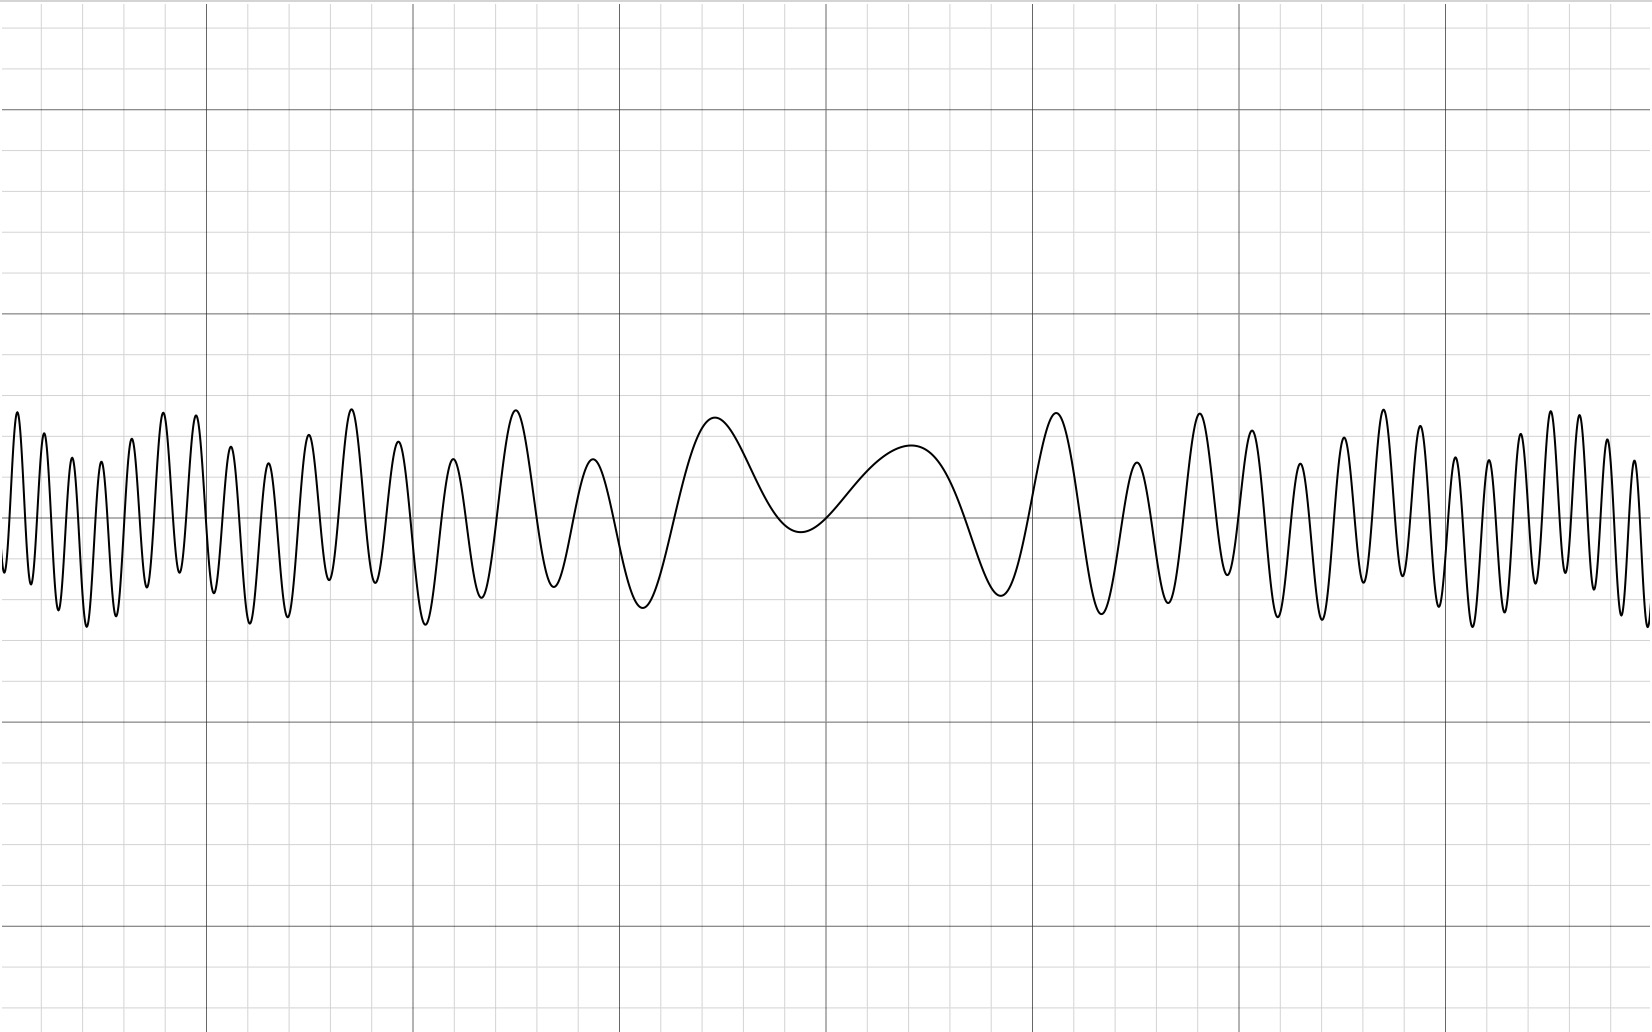
\includegraphics[height=6cm]{graph1.jpeg}
\end{center}
这很\alert{复杂}。(这里 $-10 < x < 10$.)
\end{frame}

\begin{frame}
\frametitle{换一个问题:}
在 $x = 0$ 附近,
$$ y = f(x) = \sin x^2 + \dfrac{\sin 3x}{3}$$
的图像长什么样子?比如

$$\textcolor{red}{-0.01 < x < 0.01}$$
\end{frame}

\begin{frame}
\frametitle{这样——}
\begin{center}
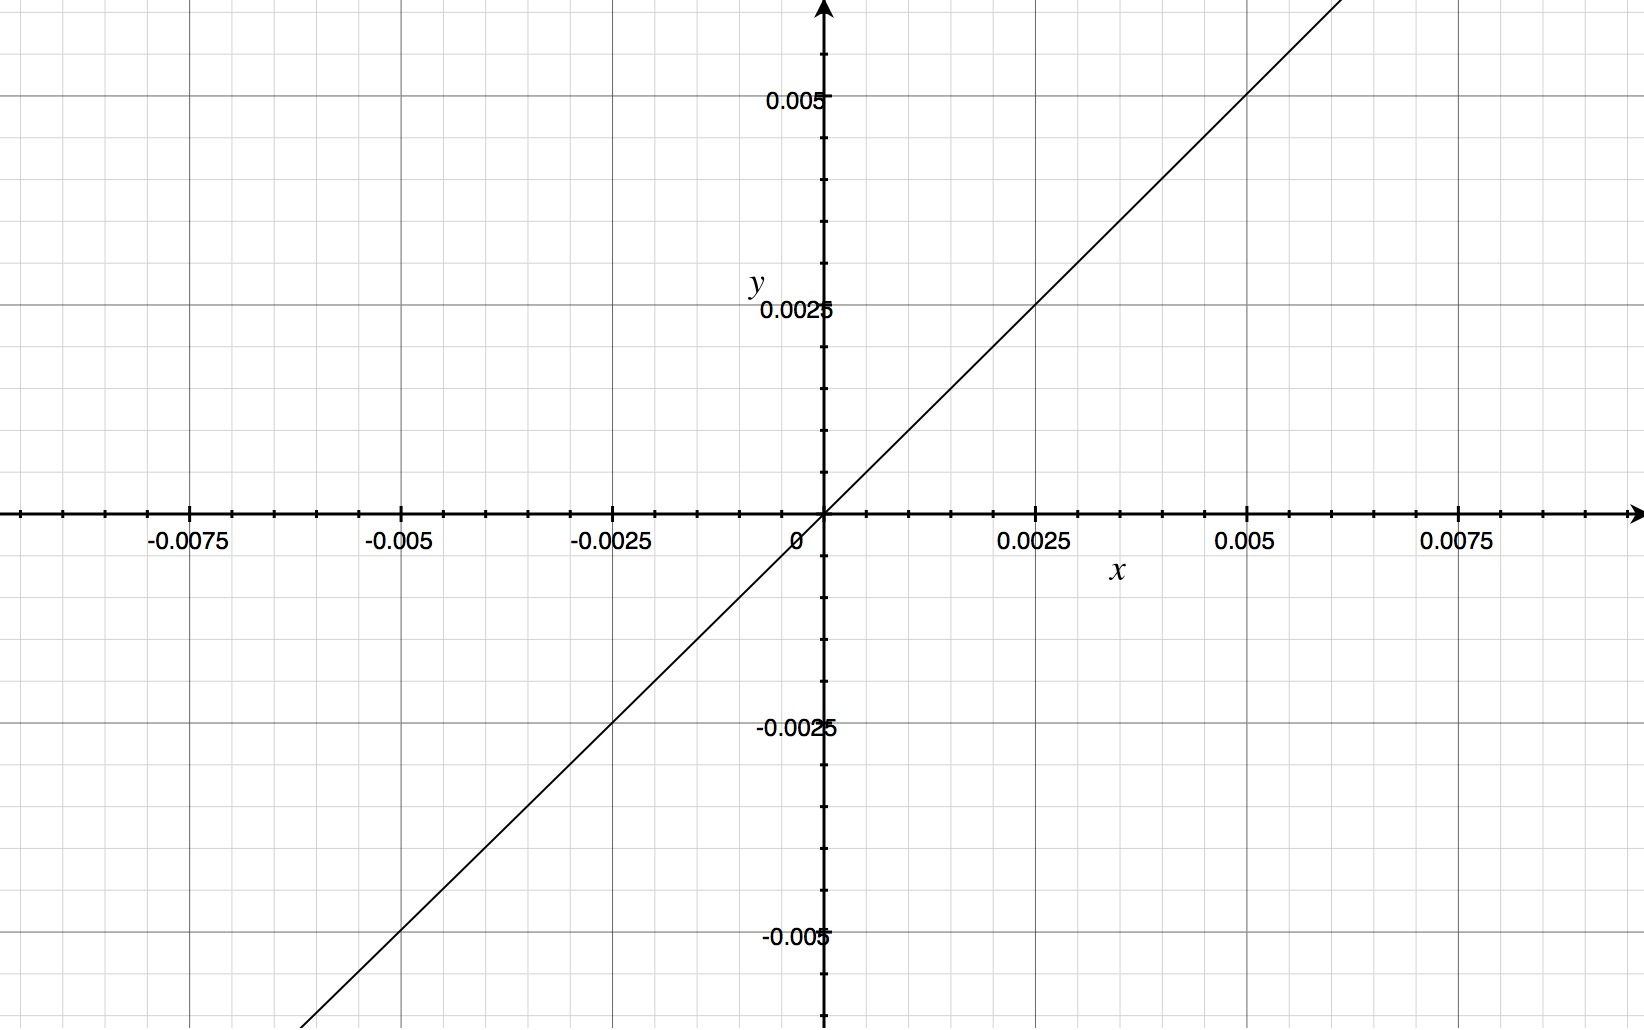
\includegraphics[height=6cm]{graph2.jpeg}
\end{center}
这很\alert{简单},(几乎)就是一条\alert{直线}。
\end{frame}

\begin{frame}
``这条''直线的\alert{斜率},就是
\begin{center}
$f(x)$ 在 $x = 0$ 这点的\alert{导数} (derivative), 记作 $f'(0)$
\end{center}

猜猜 $f'(0)$ 等于多少?
\end{frame}

\begin{frame}
\frametitle{导数的严格定义}
\[
\begin{split}
	f'(a) &= \lim_{h\to 0} \dfrac{f(a+h) - f(a)}{(a + h) - a}(\star)\\
	&= \lim_{h\to 0} \dfrac{f(a+h) - f(a)}{h} 
\end{split}
\]
$(a + h, f(a + h))$ 和 $(a, f(a))$ 是函数图像上的两点,(\star) 是他们之间连线的斜率。
取极限——$f(x)$ 在 $x = a$ 的\alert{导数},是\alert{切线的斜率}。这个值也叫 $f(x)$ 在 $x = 0$ 的\alert{变化率}。
\end{frame}

\begin{frame}
\frametitle{作为函数的导数}
导数是一个数,但它\alert{不仅仅是一个数}:

对于函数 $f(x)$, 如果它在任意一点都有导数,

则从 $f(x)$ 我们可以得到一个\alert{新的}函数 $f'(x)$:

\vspace{1em}

$f'(x)$ 在 $x = c$ 处的值,

是 $y = f(x)$ 的图像在 $(c, f(c))$ 这点的\alert{切线的斜率}。
\end{frame}

\begin{frame}
\frametitle{一个小问题}
下图中有两个函数的图像,一个是 $f(x)$,一个是 $f'(x)$,把它们区分出来。
\begin{center}
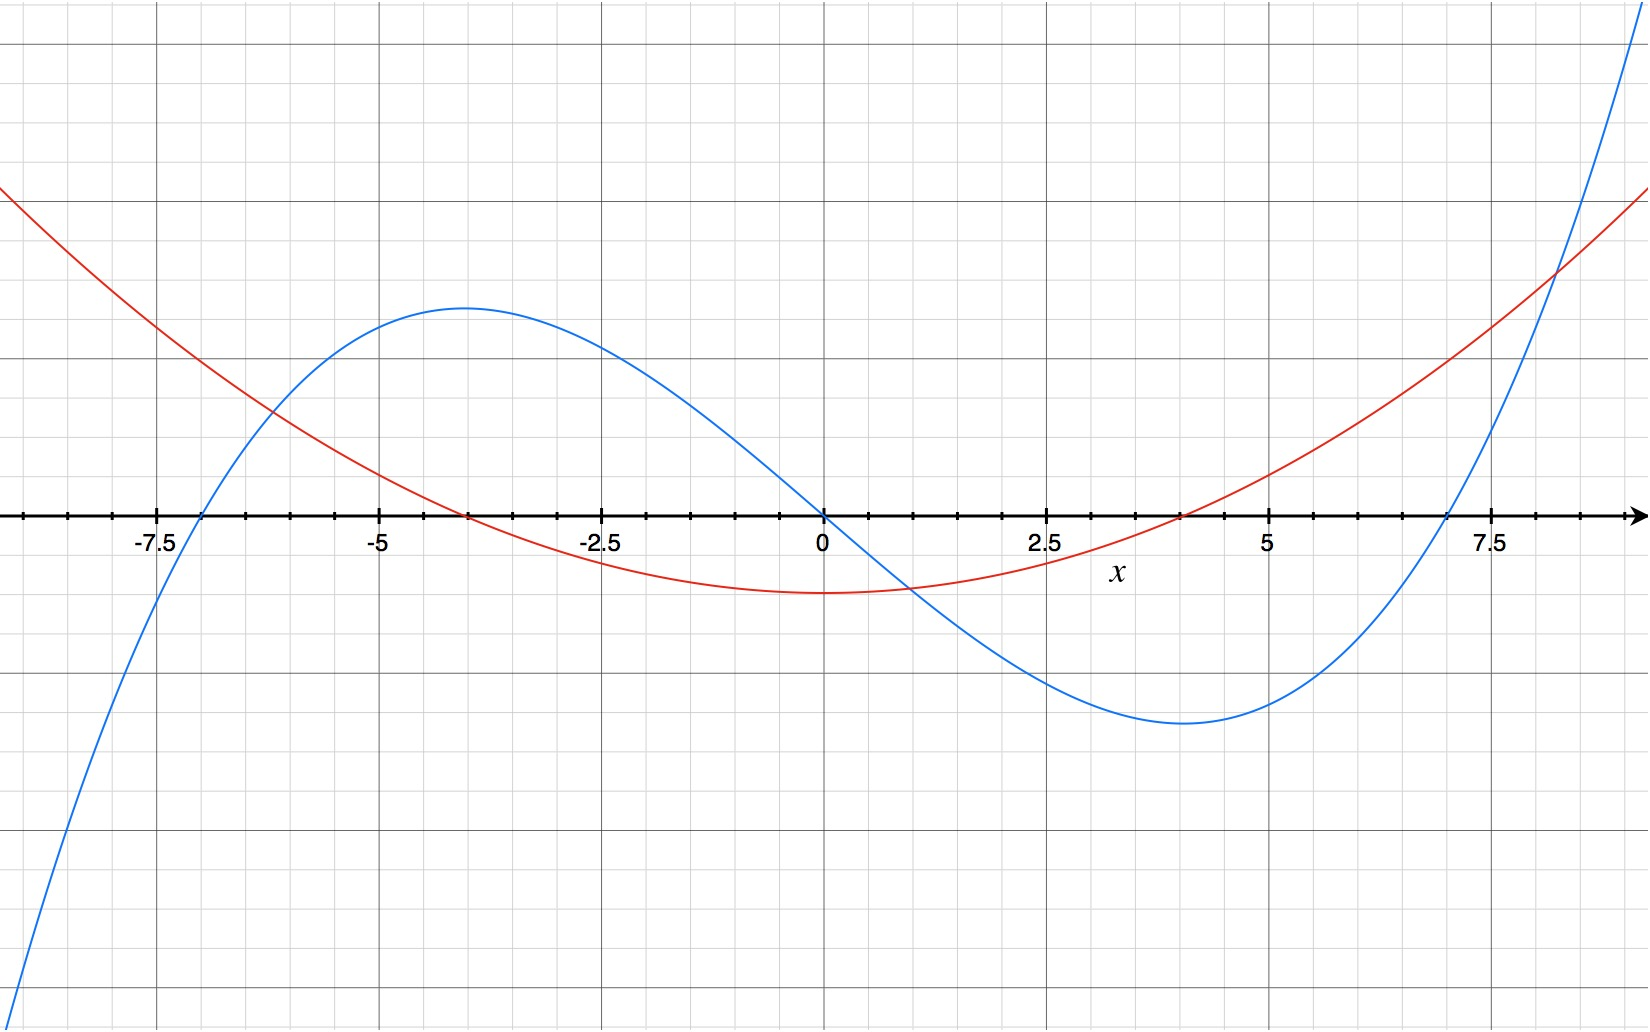
\includegraphics[height=6cm]{graph7.jpeg}
\end{center}
\end{frame}


\begin{frame}
\frametitle{罗尔定理(Rolle's Theorem)}
给定 $[a,b]$ 上的连续函数 $f(x)$, 如果 $f(x)$ 在 $(a,b)$ 上有导数,且 $f(a) = f(b) = 0$, 则存在$c\in(a,b)$ 使得 $f'(c) = 0$。
\end{frame}

\begin{frame}
\frametitle{罗尔定理(Rolle's Theorem)}
为什么罗尔定理是对的呢?

一只鸟从 $a$ 飞到 $b$, 中间肯定要经过一个\alert{最高点},最高点的切线斜率就是 $0$.
\end{frame}

\begin{frame}
\frametitle{罗尔定理(Rolle's Theorem)}
严格证明:
\begin{itemize}
	\item 如果 $f(x)$ 在 $(a, b)$ 中某点处 $> 0$,则 $f(x)$ 一定有非零的\alert{最大值},在那个点导数为 $0$.
	\item 如果 $f(x)$ 在 $(a, b)$ 中某点处 $< 0$,则 $f(x)$ 一定有非零的\alert{最小值},在那个点导数为 $0$.
	\item 如果 $f(x)$ 在 $(a, b)$ 中既不大于零,也不小于零,则 $f(x)$ \alert{总是} $0$,$(a, b)$ 中任意一点的导数都为 $0$.
\end{itemize}
\end{frame}

\begin{frame}
\frametitle{又一个小问题}
$f(x)$ 有四个零点,求证 $f'''(x)$ 有一个零点。
\end{frame}

\begin{frame}
\frametitle{面积}
给定 $[a,b]$ 上的连续函数 $f(x)$,下图阴影部分
\begin{center}
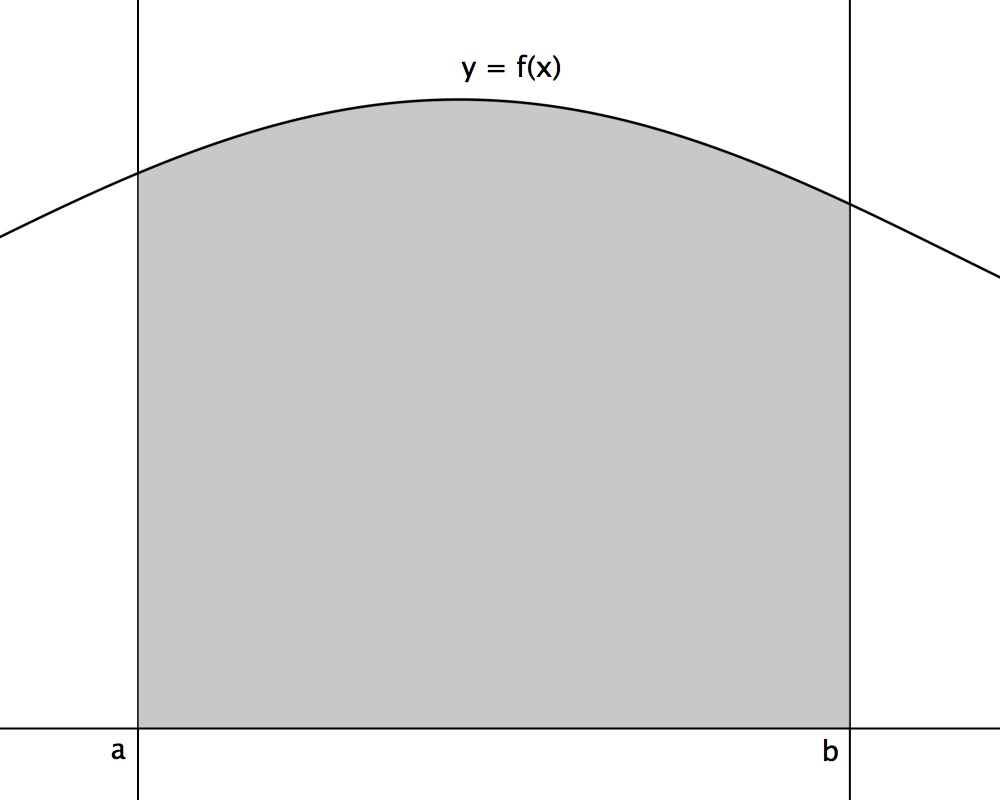
\includegraphics[height=6cm]{graph6.jpeg}
\end{center}
的面积是多少?
\end{frame}

\begin{frame}
\frametitle{面积}
为上述面积引入一个\alert{记号}
\[
	\int_a^b f(t)dt
\]
——其中真正的\alert{信息}是 $a, b, f$.

\vspace{1em}

至于 $t$, 只是一个\alert{哑变量}(dummy variable),同样的量,记作
\[
	\int_a^b f(x)dx
\]
也是可以的。这个记号读作 $f(x)dx$ 从 $a$ 到 $b$ 的\alert{积分}
\end{frame}

\begin{frame}
\frametitle{面积}

一旦克服了对新记号的\alert{恐惧},

对于$[a,b]$上的连续函数$f(x)$

这只不过是个\alert{数字}而已。

所以——以下对话也是合理的:

\begin{itemize}
	\item 你今年多大了?
	\item 我今年 $ \displaystyle\int_0^{25}\dfrac{x^3dx}{1+x^3} $ 岁。
\end{itemize}

至于怎么计算,那是\alert{另一回事}。

\end{frame}


\begin{frame}
\frametitle{一点点``哲学''}

\alert{定义与计算的分离}可以说是一个重大的飞跃。很多人就栽倒在这里。

\begin{itemize}
	\setlength\itemsep{0.5em}
	\item 定义通常\alert{有深刻的意义},但却对计算\alert{没有帮助}。
	\item 计算通常用到\alert{由定义导出的技巧},但是不理解定义直接引入,则\alert{莫名其妙}。
	\item 单纯\alert{做题}(通常是计算)有时无助于理解定义。
	\item 需要\alert{沉思}。
\end{itemize}

\end{frame}


\begin{frame}
\frametitle{黎曼和(Riemann Sum)}
积分的真正定义
\[
	\int_a^b f(x)dx := \lim_{|\Delta|\to 0}\sum_i f(x_i^*)\Delta x_i
\]

完全\alert{无助于}计算,但却对\alert{理解}积分非常重要。
\end{frame}

\begin{frame}
\frametitle{黎曼和(Riemann Sum)}
上面右边的求和,叫做\alert{黎曼和},这是一些矩形的面积之和
\begin{center}
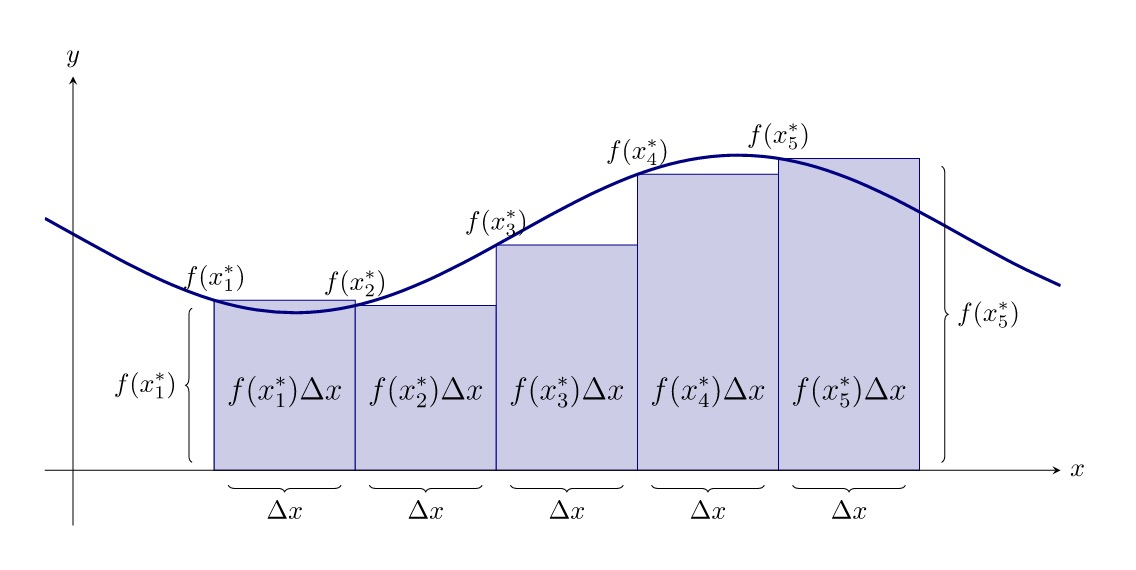
\includegraphics[height=5cm]{graph9.jpeg}
\end{center}
\[
f(x_1^*)\Delta x_1 + f(x_2^*)\Delta x_2 + \cdots + f(x_5^*)\Delta x_5 =: \sum_{i=1}^5 f(x_i^*)\Delta x_i
\]
\end{frame}

\begin{frame}
\frametitle{黎曼和(Riemann Sum)}
对于更细的划分$\Delta$,显然,这个和要更接近曲线下方的面积
\begin{center}
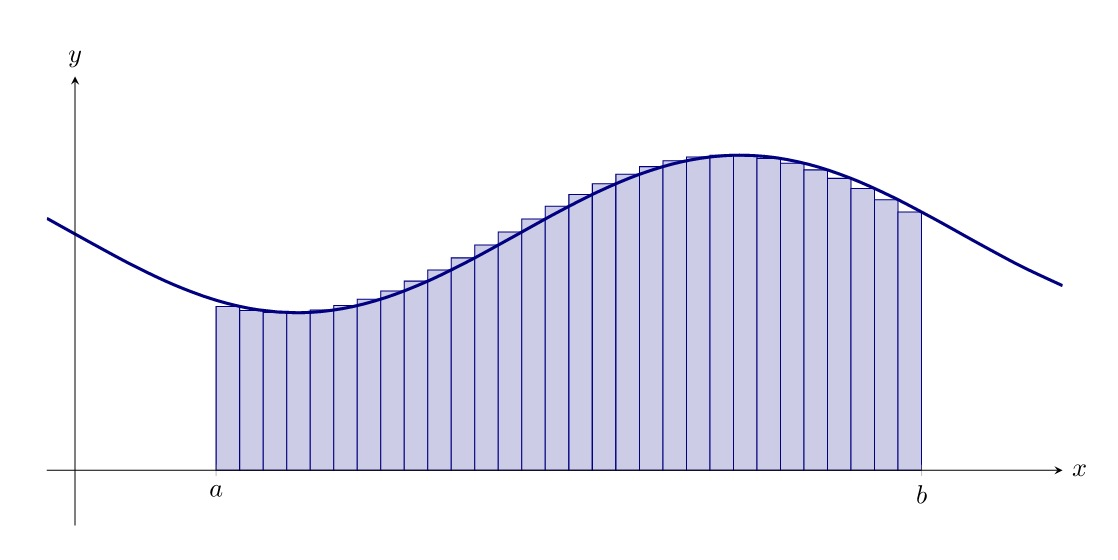
\includegraphics[height=5cm]{graph10.jpeg}
\end{center}
\[
f(x_1^*)\Delta x_1 + f(x_2^*)\Delta x_2 + \cdots + f(x_n^*)\Delta x_n =: \sum_{i=1}^n f(x_i^*)\Delta x_i
\]
\end{frame}

\begin{frame}
\frametitle{黎曼和(Riemann Sum)}
取极限
\[
	\lim_{|\Delta|\to 0}\sum_i f(x_i^*)\Delta x_i
\]

就是(黎曼)积分的\alert{定义}:
\[
	\int_a^b f(x)dx := \lim_{|\Delta|\to 0}\sum_i f(x_i^*)\Delta x_i
\]
\end{frame}

\begin{frame}
\begin{center}
\frametitle{一个自然的问题}
道理我都懂,那到底怎么\alert{计算}刚刚定义出来的面积呢?
\end{center}

\end{frame}

\begin{frame}
\frametitle{牛顿-莱布尼兹公式}
一个神奇的公式

又叫``微积分基本定理''(fundamental theorem of calculus):
\[
	\dfrac{d}{dx}\int_a^x f(t)dt = f(x)
\]
左边 = 面积的变化率,右边 = 函数$f(x)$的值。

这是一个\alert{不平凡}的公式,但它\alert{显然}是对的,为什么呢?
\end{frame}

\begin{frame}
\begin{center}
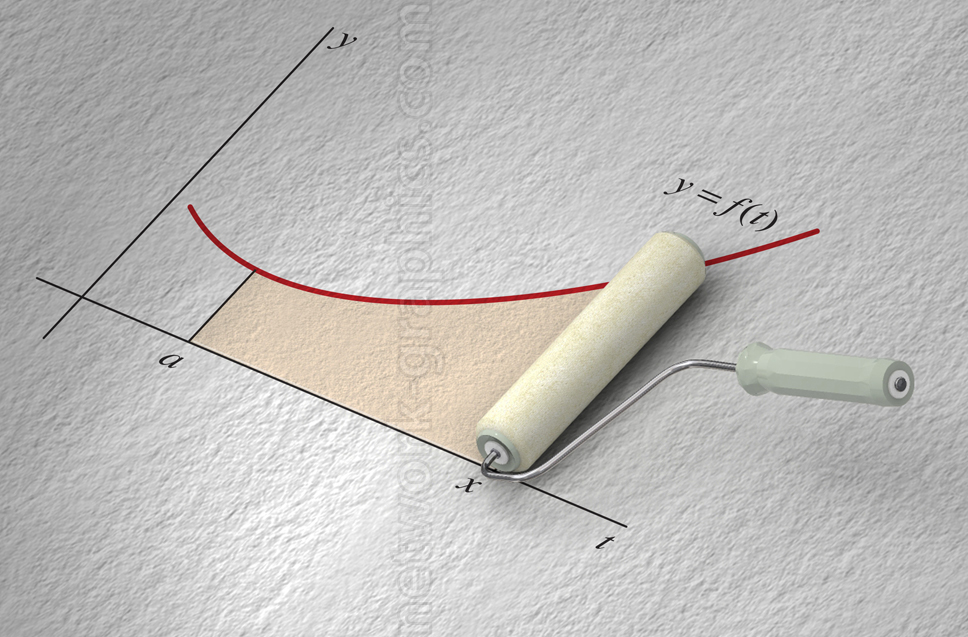
\includegraphics[height=7cm]{paintroller_area_m.jpg}
\end{center}
\end{frame}

\begin{frame}
\begin{center}
因为面积的变化率就是函数在那一点的值啊。
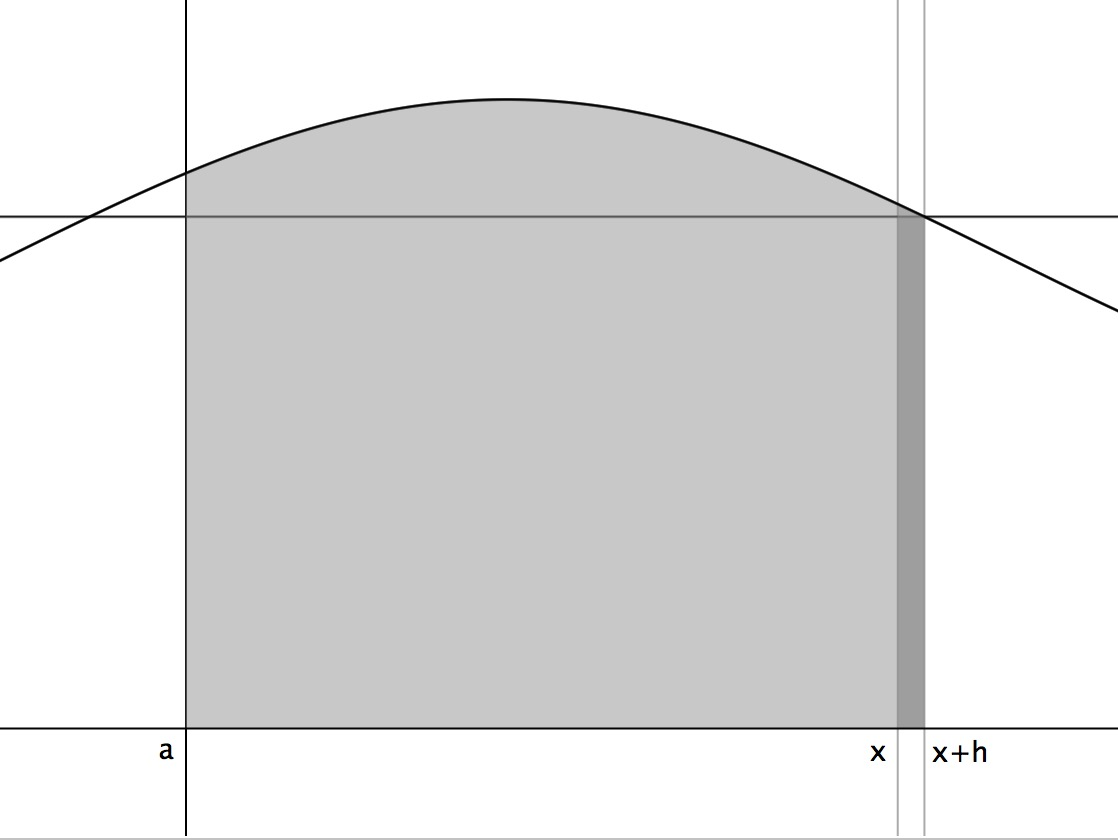
\includegraphics[height=6cm]{graph3.jpg}
\end{center}
\end{frame}

\begin{frame}
\frametitle{面积的变化率}
如果把面积 $\displaystyle\int_a^x f(t)dt$ 记作 $F(x)$, 则\alert{按照定义},面积的变化率为
\[
	\dfrac{dF(x)}{dx} = \lim_{h\to 0}\dfrac{F(x+h) - F(x)}{h}
\]
\end{frame}

\begin{frame}
\frametitle{面积的变化率}
右边的分子,是两块面积的差,也就是下图中阴影部分的值
\begin{center}
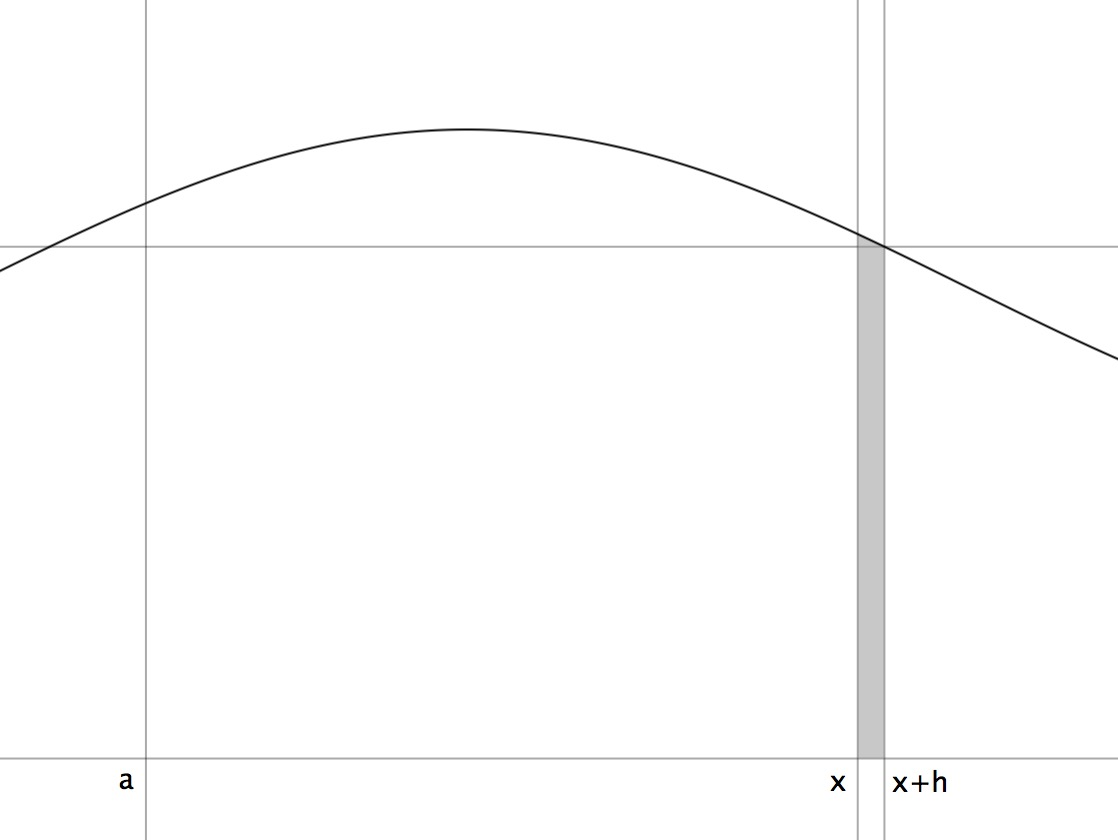
\includegraphics[height=6cm]{graph4.jpeg}
\end{center}
\end{frame}

\begin{frame}
\frametitle{面积的变化率}
如果把阴影部分看作下图的\alert{矩形},则矩形面积等于底乘以高——底边长为 $h$,而高正好是 $f(x)$。
\begin{center}
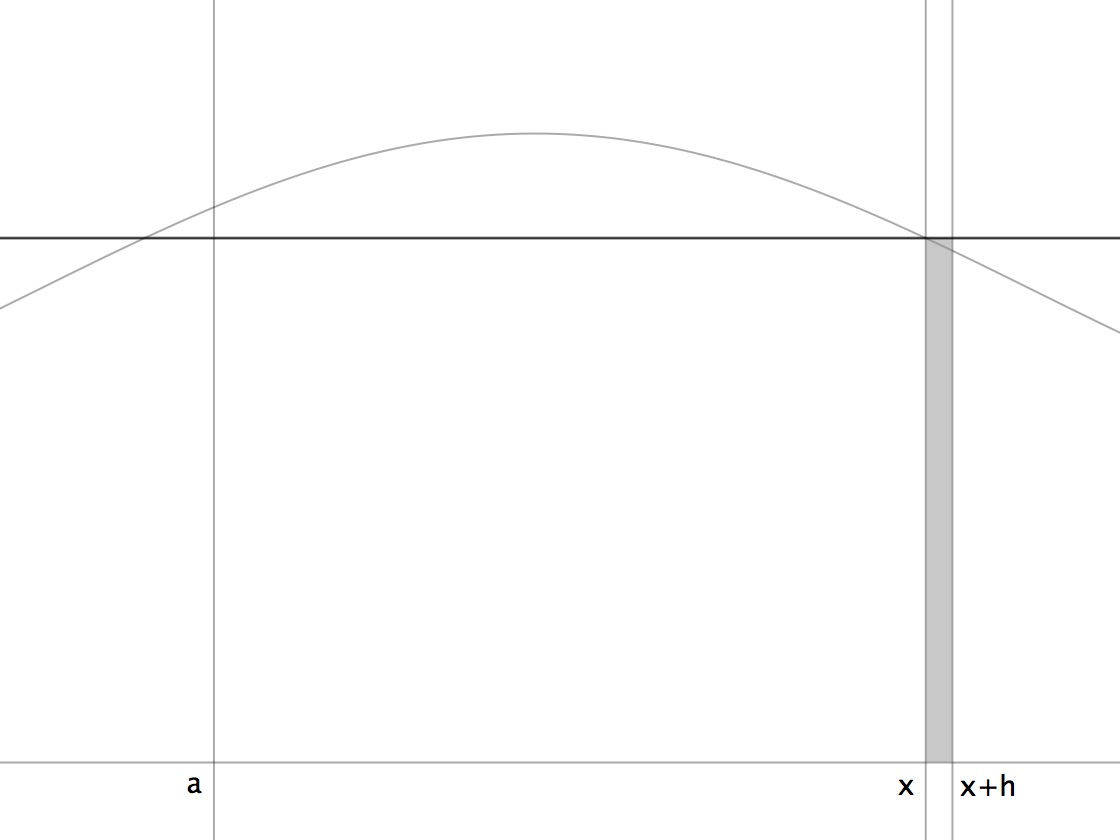
\includegraphics[height=6cm]{graph5.jpeg}
\end{center}
\end{frame}

\begin{frame}
\frametitle{定积分}
牛顿-莱布尼兹公式到底告诉我们什么呢?

一件困难的事情——计算\alert{黎曼和的极限},
\[
	\int_c^d f(x)dx := \lim_{|\Delta|\to 0}\sum_i f(x_i^*)\Delta x_i
\]
可以转化成一件简单的事情——计算\alert{一个函数在两点的取值的差}。
\[
	\int_c^d f(x)dx = F(c) - F(d)
\]
只要你能\alert{找到}一个 $F(x)$ 使得 $F'(x) = f(x)$.
\end{frame}

\begin{frame}
\frametitle{辅助工具}
\begin{center}

\includegraphics[height=5cm]{graph8.jpeg}
\end{center}
这个 App 接受输入
``integral of x/(1+x\^{}3)dx for x from 1 to 10''

网站 \url{www.wolframalpha.com} 也有类似的功能。 
\end{frame}

\begin{frame}
\frametitle{图片来源}
\begin{itemize}
	\item 黎曼和的两张图片来自 \url{https://ximera.osu.edu/course/mooculus/mooculus/textbook/approximatingTheAreaUnderACurve/digInApproximatingAreaWithRectangles}
	\item 牛顿-莱布尼兹公式后面那张刷油漆的图片来自 \url{http://www.network-graphics.com/images/calculus/paintroller_area_m.jpg}
\end{itemize} 
\end{frame}

\end{document}